% ---------------------------------------------------%
% DISCLAIMER: ADA KEMUNGKINAN BAB 3 STRUKTUR YG DIBAHAS BERBEDA, JADI DI BAWAH ADA CONTOH
% BAB 3 KATING. MODIF SAJA SESUAI KEBUTUHAN

% ---------------------------------------------------%

% \chapter{Analisis dan Perancangan}
\chapter{Analisis Masalah dan Solusi}

\section{Analisis Masalah}
\label{sec:analisis-masalah}

Protokol komunikasi pada dasarnya dibangun untuk melayani komunikasi data antara dua buah pihak yang berbeda. Hal ini sesuai syarat jaringan komputer yang telah dijelaskan pada bagian \ref{sec:jaringan-komputer}. Protokol komunikasi harus dapat memastikan pesan yang dikirimkan dapat diterima oleh pihak penerima pesan serta dipahami isinya. Selain itu, protokol komunikasi juga harus memastikan ancaman apabila terdapat pihak ketiga yang terlibat baik secara aktif ataupun pasif. Selain itu, penerapan enkripsi dinamis pada sistem \emph{chaos} menimbulkan beberapa masalah kompatibilitas. Oleh karena itu, terdapat beberapa permasalahan yang akan dibahas pada bagian ini. Secara garis besar, permasalahan yang muncul ditunjukan pada tabel \ref{tab:permasalahan}.

\begin{table}[!h]
  \centering
  \caption{Permasalahan yang dihadapi pada protokol TLS dengan \emph{Cipher} berbasis sistem \emph{chaos}} \label{tab:permasalahan}
  \begin{tabular}{|c|p{6cm}|p{4cm}|}
    \hline
    \textbf{ID Masalah} & \textbf{Deskripsi} & \textbf{Rumusan Masalah Terkait} \\
    \hline
    P1 & Pemilihan Versi Protokol TLS & 2 \\ \hline
    P2 & Serangan MITM saat adanya komunikasi berlangsung & 2 \\ \hline
    P3 & Serangan \emph{replay attack} saat adanya komunikasi berlangsung & 1 dan 2 \\ \hline
    P4 & Serangan \emph{tampering} pada pesan terenkripsi & 2 \\ \hline
    P5 & Serangan kriptografi melalui analisis pesan terenkripsi & 1 \\ \hline
    P6 & Ancaman analisis nilai acak yang dihasilkan oleh sistem \emph{chaos} & 1 \\ \hline
    P7 & Pembentukan nilai awal sistem \emph{chaos} & 1 dan 2 \\ \hline
    P8 & Pembentukan kunci blok baru saat proses enkripsi dan dekripsi & 1 dan 2 \\ \hline
  \end{tabular}
\end{table}

\subsection{Ancaman Keamanan pada Protokol Komunikasi}
\label{sec:ancaman-keamanan}

Pihak ketiga mungkin terlibat dalam komunikasi baik secara aktif maupun pasif. Hal ini dapat menimbulkan beberapa ancaman keamanan yang ada pada protokol komunikasi. Bagian ini akan menjelaskan rincian analisis ancaman keamanan yang dihadapi oleh protokol ini. Untuk mempermudah penjelasan, diasumsikan terdapat dua buah pihak yang melakukan komunikasi, yaitu Ahmad dan Budi. Terdapat pihak ketiga dalam komunikasi bernama Candra sebagai pihak yang tidak berhak terlibat dalam komunikasi. 

Dalam komunikasi, memungkinkan Candra mengaku sebagai salah satu pihak yang terlibat dalam komunikasi, yaitu Ahmad dan Budi. Hal ini dapat dilakukan dengan melakukan serangan MITM di antara kedua belah pihak. Dengan melakukan serangan ini, memungkinkan Candra mendapatkan informasi yang dikirimkan oleh Ahmad dan Budi. Oleh karena itu, perlu adanya mekanisme untuk memastikan bahwa pihak yang terlibat merupakan pihak yang dipercaya.

Selain itu, Candra juga dapat melakukan serangan berupa \emph{replay attack}. Dalam serangan ini, Candra bertujuan untuk mengganggu sistem dengan mengirimkan ulang pesan-pesan tertentu yang telah direkam. Candra mungkin tidak dapat mengetahui isi dari data yang ada pada \emph{frame}, tetapi \emph{frame} tersebut dapat menyebabkan efek yang tidak diinginkan oleh Ahmad ataupun Budi. Oleh karena itu, perlu adanya otentikasi partisipan pada pesan.

Dalam komunikasi, Candra dapat mengubah \emph{frame} yang dikirimkan oleh Ahmad ataupun Budi. Hal ini dapat menyebabkan pesan yang dikirimkan tidak dapat dipahami oleh penerima. Selain itu, hal ini dapat memberikan efek yang tidak diinginkan oleh penerima, seperti serangan \emph{bit flip}. Oleh karena itu, perlu adanya mekanisme untuk menjaga integritas pesan yang dikirimkan oleh Ahmad ataupun Budi.

Pesan yang dikirimkan dalam jaringan publik dapat diamati oleh Candra. Candra dapat mengetahui isi pesan terenkripsi yang telah dikirimkan oleh Ahmad ataupun Budi. Hal ini dapat dicapai dengan melakukan beberapa teknik diantaranya adalah melakukan \emph{brute force} terhadap kunci enkripsi. Teknik lainnya yang dapat dilakukan oleh Candra adalah melakukan analisis teks enkripsi. Salah satu teknik yang bisa dilakukan adalah melakukan analisis berbasikan \emph{plaintext} yang telah diketahui. Candra dapat mengamati pola yang dibentuk dari hasil enkripsi. Candra juga dapat melakukan analisis terhadap \emph{ciphertext} yang telah diterima. Hal ini dapat dilakukan dengan melakukan analisis frekuensi terhadap blok pesan ataupun melakukan analisis secara visual terhadap \emph{ciphertext}. Harapan dari proses ini mendapatkan pola dari \emph{ciphertext} sehingga dapat dianalisis apa isi pesan yang terenkripsi.

\subsection{Analisis Permasalahan Penerapan AES dengan Sistem \emph{Chaos} pada Protokol TLS}
\label{sec:ancaman-implementasi}
Dalam penerapan \emph{cipher} AES dengan sistem \emph{chaos} pada protokol TLS, diperlukan memilih versi protokol TLS yang tepat. Pemilihan versi protokol TLS yang tepat perlu memperhatikan keamanan yang diberikan oleh protokol tersebut. Pada dasarnya, protokol TLS memiliki beberapa versi yang berbeda, diantaranya adalah TLSv1.0, TLSv1.1, TLSv1.2, dan TLSv1.3. 

Selain itu, sistem \emph{chaos} yang tepat perlu dipilih untuk digunakan sebagai kunci blok. Sistem \emph{chaos} ini juga harus memiliki sifat \emph{forward unpredictability} dan \emph{backward unpredictability} sebagaimana yang dijelaskan pada bagian \ref{sec:nist.statistical.test}. Ancaman yang terkait dengan hal ini adalah adanya analisis nilai acak untuk mendapatkan nilai acak yang akan datang dan nilai acak yang telah digenerate sebelumnya. Hal ini dapat menyebabkan pesan yang dikirimkan dapat didekripsi oleh penyerang, baik pesan yang diterima dan pesan yang akan datang.

Sistem \emph{chaos} juga memerlukan nilai awal atau \emph{seed} yang akan digunakan sebagai nilai awal dari sistem \emph{chaos}. Nilai ini perlu dihasilkan dari proses \emph{handshake} yang dilakukan melalui protokol TLS. Oleh karena itu, diperlukan sebuah mekanisme pembangkitan nilai \emph{seed} melalui prosedur \emph{handshake} tersebut.

Pada protokol TLS berbasis chaos, kunci blok yang digunakan bersifat dinamis. Hal ini memerlukan analisis lebih lanjut terkait metode pembaharuan kunci blok yang digunakan pada protokol ini pada masing-masing pihak. Hal ini diperlukan agar \emph{state} dari kunci blok dapat terjamin.

Pada protokol TLS, terdapat mekanisme pemeriksaan integritas pesan. Mekanisme ini memanfaatkan MAC yang dienkripsi bersama pesan. Ancaman dari mekanisme ini adalah adanya serangan dengan mengirimkan pesan yang tidak sah. Pembangkitan nilai acak pada sistem \emph{chaos} dinilai cukup berat sehingga bila ancaman ini terjadi, penerima dapat kehabisan \emph{resource} dalam melakukan dekripsi. Oleh karena itu, perlu adanya mekanisme untuk melakukan mekanisme pemeriksaan integeritas pesan yang diterima yang lebih efisien.

\section{Analisis Solusi}

Bagian ini akan menjelaskan terkait solusi dari permaslahan yang telah dipaparkan sebelumnya. Bagian ini akan dibagi menjadi beberapa kategori, diantaranya adalah solusi terkait dengan proses sistem chaos, sinkronisasi sistem chaos, proses enkripsi dan dekripsi, dan proses otentikasi pengirim pesan. Secara garis besar, solusi yang diusulkan ditunjukkan pada tabel \ref{tab:solusi}.

\begin{table}[!h]
  \centering
  \caption{Solusi yang diusulkan pada protokol yang diusulkan} \label{tab:solusi}
  \begin{tabular}{|c|p{6cm}|c|}
    \hline
    \textbf{ID Solusi} & \textbf{Deskripsi} & \textbf{Permasalahan Terkait} \\
    \hline
    S1 & Menggunakan sistem chaos berbasis \emph{Sine-Henon map} untuk pembangkit bilangan acak & P5 dan P6 \\ \hline
    S2 & Pertukaran Kunci menggunakan Diffie-Hellman & P7 \\ \hline
    S3 & Proses pembangkitan \emph{state} awal sistem \emph{chaos} dilakukan dari proses TLS Handshake & P7 \\ \hline
    S4 & Cipher yang digunakan adalah AES dengan blok CTR dan kunci blok dinamis berbasiskan sistem chaos \emph{Sine-Henon map} & P3 dan P5 \\ \hline
    S5 & Mekanisme pengubahan kunci enkripsi dan dekripsi & P8 \\ \hline
    S6 & Pesan terenkripsi dilindungi oleh MAC yang melibatkan nomor frame & P4 \\ \hline
    S7 & Parameter Diffie-Hellman harus ditandatangani melalui tanda tangan digital & P2 \\ \hline
    S8 & Mekanisme pemeriksaan tanda tangan digital & P2 \\ \hline
    S9 & Melakukan implementasi pada protokol TLSv1.2 & P1, P2, P4, dan P4 \\ \hline
    S10 & Melakukan implementasi pemeriksaan \emph{certificate} pada sisi klien & P2 \\ \hline
  \end{tabular}
\end{table}

\subsection{Sistem Chaos}

Pada penelitian yang dilakukan oleh \textcite{lin2021}, sistem chaos yang digunakan adalah sistem chaos berbasis Hénon Map. Nilai hasil pembangkitan diambil melalui parameter $X_n$ yang dihasilkan pada setiap iterasi. Bila diamati melalui persamaan \ref{eq:chaos.henon}, bila diketahui nilai $X_n$, akan sangat sulit untuk mendapatkan nilai $X_{n-1}$ dikarenakan diperlukannya nilai $Y_n$ yang tidak diketahui. Oleh karena itu, sistem chaos ini sukar untuk dilakukan \emph{backward predictability}. Kelemahan dari sistem \emph{chaos} ini adalah sistem ini masih dapat dilakukan \emph{forward predictability} bila dua nilai berurutan yang dihasilkan oleh sistem \emph{chaos} dapat diketahui. 

Hal ini dapat diperbaiki dengan melibatkan sistem chaos lain berbasis \emph{sine map}. Sistem chaos berbasis \emph{sine map} dipilih dikarenakan sistem chaos ini menghasilkan titik diantara $0$ dan $1$ sehingga memudahkan dalam melakukan konversi dalam byte. Selain itu, nilai diantara $0$ dan $1$ juga memiliki kepadatan yang cukup baik bila diinterpretasikan pada \emph{floating point} sehingga diharapkan dapat menghasilkan nilai acak yang lebih banyak.

Peraduan antara sistem chaos berbasis \emph{sine map} dan sistem chaos berbasis Hénon Map dapat dilakukan seperti metode yang dijelaskan oleh \textcite{patel2021}. Dari hasil tersebut, dapat dibentuk sistem \emph{chaos} baru yang disebut SineHenonMap yang didefinisikan pada persamaan \ref{eq:tls.chaos}.

\begin{equation}
  \begin{aligned}
    X_{i+1} = \text{mod}((1 - a \cdot X_i^2 + Y_i) + (\frac{\mu}{4} \cdot \sin{(\pi \cdot X_{i})}) \cdot 100, 1)  \\
    Y_{i+1} = \text{mod}((b \cdot X_i + Z_{i}) \cdot 100, 1) \\
    Z_{i+1} = \frac{\mu}{4} \cdot \sin{(\pi \cdot Z_{i})}
  \end{aligned}
  \label{eq:tls.chaos}
\end{equation}

Pada persamaan \ref{eq:tls.chaos}, terdapat pengali dengan nilai $100$. Nilai ini digunakan untuk memperoleh distribusi \emph{uniform} pada nilai yang dihasilkan sebagaimana yang dilakukan oleh \textcite{nurhaliza2023}. Hal ini diilustrasikan pada gambar \ref{fig:chaos.sinehenonmap.dist}. Pemilihan nilai $\mu$ yang digunakan adalah $3.75$ dan $a$ serta $b$ adalah $1.4$ dan $0.3$. Hal ini diambil berdasarkan nilai yang digunakan pada penelitian \textcite{lin2021} dan \textcite{patel2021}. Prasayat dari sistem chaos pada persamaan \ref{eq:tls.chaos} adalah nilai $X_0$, $Y_0$, dan $Z_0$ harus berada pada range $(0,1)$. Hal ini dilakukan untuk menjamin kepadatan nilai yang dihasilkan oleh sistem \emph{chaos}.

\begin{figure}[!h]
  \centering
  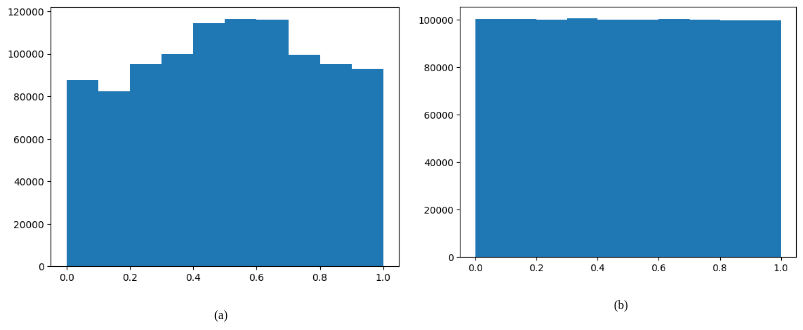
\includegraphics[width=400px]{chapters/res/chapter-3/img/sinehenon.distribution.png}
  \caption{Distribusi nilai dari sistem chaos Sine-Hénon Map (a) tanpa pengali dan (b) dengan pengali} \label{fig:chaos.sinehenonmap.dist}
\end{figure}

\subsection{Sinkronisasi Sistem Chaos}

Menurut \textcite{lin2021}, sinkronisasi sistem \emph{chaos} dapat dilakukan dengan memanfaatkan \emph{sliding mode control}. Namun, metode ini memerlukan RTT yang cukup banyak untuk melakukan sinkronisasi. Pada protokol TLS, pada dasarnya telah disediakan mekanisme untuk pertukaran kunci dengan melalui proses \emph{handshake}. Oleh karena itu, sinkronisasi sistem \emph{chaos} dapat dilakukan dengan memanfaatkan \emph{master key} dari proses tersebut.

Permasalahan selanjutnya adalah terkait dengan konversi nilai bilangan bulat menjadi nilai \emph{state} pada sistem \emph{chaos}. Prasayat dari sistem \emph{chaos} pada persamaan \ref{eq:tls.chaos} adalah nilai $X_0$, $Y_0$, dan $Z_0$ harus berada pada range $(0,1)$. Oleh karena itu, proses konversi dapat dilakukan dengan melakukan ekspansi kunci setidaknya $3n$ bit nilai. Selanjutnya, nilai tersebut dilakukan perbandingan nilai pada blok hasil ekspansi kunci dengan nilai maksimum blok tersebut. Hal ini dinyatakan pada persamaan \ref{eq:tls.convert}.

\begin{equation}
  \begin{aligned}
    f(K) = \frac{K}{2^{n}} \\
  \end{aligned}
  \label{eq:tls.convert}
\end{equation}

Dalam hal ini nilai $n$ adalah jumlah bit maksimum. Pada protokol yang dibangun, jumlah bit yang diambil adalah $n = 256$. Hal ini didasari dengan tipe data float memiliki ketelitian yang cukup baik pada 32 bit.

Protokol TLS pada dasarnya mendukung dua tipe pertukaran kunci seperti yang telah dijelaskan pada \emph{sec:tls.keyexchange}. Pertukaran kunci yang cocok untuk diterapkan pada sistem \emph{chaos} adalah pertukaran kunci dengan memanfaatkan protokol Diffie-Hellman. Hal ini dikarenakan protokol ini memiliki keamanan yang lebih tinggi dibandingkan RSA. Selain itu, keteracakan dihasilkan juga oleh kedua buah pihak yang terlibat sehingga keteracakan tidak hanya tergantung oleh satu pihak. Hal ini sesuai dengan prinsip \emph{defense in depth} pada keamanan data.


\subsection{Enkripsi dan Dekripsi Pesan}
\label{sec:solusi.enc-dec}

Pada saat proses enkripsi ataupun dekripsi pesan, diperlukan bit-bit kunci yang dibangkitkan melalui sistem \emph{chaos}. Proses pengubahan titik \emph{chaos} pada persamaan \ref{eq:tls.chaos} menjadi bilangan bulat dapat dilakukan persamaan \ref{eq:tls.convert.int}.

\begin{equation}
  \begin{aligned}
    K_i = \lfloor{X_i \cdot 2^{n}}\rfloor
  \end{aligned}
  \label{eq:tls.convert.int}
\end{equation}

Proses pengubahan ini diambil dikarenakan $K_i$ yang dihasilkan akan langsung berada pada jumlah bit yang dibutuhkan. Hal ini dapat menghemat operasi yang diperlukan dalam melakukan konversi. Nilai $K_i$ yang dihasilkan akan digunakan sebagai kunci blok yang digunakan pada proses enkripsi dan dekripsi.

Algoritma yang digunakan untuk proses enkripsi dan dekripsi adalah AES-256. Algoritma enkripsi ini dikarenakan dukungan terhadap algoritma ini sudah sangat baik pada berbagai sistem. Selain itu, kekuatan dari AES-256 sampai saat ini masih sangat baik. Algoritma ini juga dapat dijalankan pada berbagai perangkat dengan kecepatan yang baik dengan adanya bantuan microprocessor yang mendukung instruksi AES.

Permasalahan selanjutnya adalah terkait dengan sistem blok yang digunakan. Pada protokol yang dibangun, sistem blok yang digunakan adalah mode CTR. Mode CTR dapat memberikan fleksibilitas dalam pembentukan kunci dikarenakan proses enkripsi dan dekripsi keduanya dapat dilakukan secara parallel. Selain itu, mode CTR dapat diubah dengan mudah menjadi cipher alir sehingga dapat digunakan untuk mengirimkan aliran pesan yang terenkripsi. Mode sistem CTR juga dapat mengaburkan hubungan antar blok dikarenakan blok akan dienkripsi dengan blok CTR yang berbeda-beda.

Nilai \emph{counter} pada sistem blok CTR dibangun juga memanfaatkan sistem \emph{chaos}. Hal ini ditujukan untuk menambah keamanan dari enkripsi blok. Selain itu, menambahan sistem \emph{counter} ini juga memperpanjang orde dari kunci yang digunakan. Hal ini dapat memperbesar ruang kunci saat melakukan XOR. Oleh karena itu, upaya analisis terhadap pesan akan semakin sulit.

Permasalahan terkait dengan pembaharuan kunci blok dapat diselesaikan dengan memberikan aturan terkait dengan pembaharuan kunci. Untuk kunci enkripsi, pembaharuan kunci dilakukan setelah proses enkripsi berhasil. Hal ini cukup untuk dilakukan karena frame yang terenkripsi dapat dilakukan \emph{cache} apabila dibutuhkan retransmisi ulang. Selain itu, pembaharuan kunci segera juga mencegah kunci yang digunakan untuk enkripsi diambil oleh penyerang untuk melakukan dekripsi pesan yang telah dienkripsi sebelumnya. Untuk pengubahan nilai \emph{counter}, dapat dilakukan setelah proses enkripsi selesai. Hal ini untuk memastikan nilai \emph{counter} berubah hanya saat proses enkripsi berhasil. 

Permasalahan selanjutnya adalah terkait dengan pengubahan nilai kunci saat proses dekripsi. Perubahan kunci hanya boleh dilakukan saat MAC pesan yang diterima benar dan proses dekripsi berhasil. Hal ini untuk memastikan bahwa pesan yang diterima merupakan pesan yang benar. Pengubahan nilai counter hanya boleh dilakukan saat proses dekripsi berhasil. Hal ini untuk memastikan bahwa nilai counter yang digunakan merupakan nilai yang benar. Saat melakukan proses dekripsi, nilai awal dari sistem \emph{chaos} harus disimpan terlebih dahulu. Hal ini diperlukan untuk melakukan operasi \emph{rollback} apabila terjadi kegagalan saat melakukan dekripsi.

Permasalahan selanjutnya adalah terkait kegagalan saat melakukan proses dekripsi pada pesan yang diterima. Kondisi ini terjadi dengan dua kemungkinan, yaitu nilai MAC salah dan padding pesan salah. Apabila pesan yang diterima memiliki nilai padding salah, maka proses dekripsi dapat langsung dibatalkan saja sehingga proses komunikasi masih dapat dilanjutkan. Apabila pesan yang diterima memiliki nilai MAC yang salah, nilai state enkripsi harus dipulihkan ke nilai sebelum melakukan operasi. Oleh karena itu, perlu adanya penanganan hal tersebut.

Permasalahan terkait dengan \emph{replay attack} pada dasarnya sudah teratasi dengan mekanisme MAC pada TLS. Pada protokol TLS, perhitungan nilai MAC didasari juga dengan nomor frame. Oleh karena itu, pesan sudah terlindungi dari ancaman tersebut.

Permasalahan terkait dengan integritas pesan telah terjamin dengan adanya MAC yang digunakan. MAC dapat memastikan bahwa pesan yang diterima merupakan pesan yang asli dan otentik. Oleh karena itu, permasalahan terkait dengan integritas pesan telah teratasi.

\subsection{Otentikasi Pengirim Pesan}

Pada protokol TLS, telah terdapat mekanisme otentikasi pengirim pesan. Mekanisme ini dilakukan saat proses \emph{handshake} dan juga saat proses pengiriman berlangsung. Pada proses \emph{handshake}, terdapat proses penandatanganan digital pada parameter pertukaran kunci. Hal ini menjamin bahwa pihak yang dapat menghasilkan kunci hanyalah pihak yang benar. Penandatanganan parameter pertukaran kunci juga dapat mencegah adanya MITM attack karena nilai parameter pertukaran tersebut akan dapat diketahui apabila terjadi pengubahan.

Tanda tangan digital tersebut dibuktikan dengan data terkait sertifikat digital yang dikirimkan. Hal ini memastikan hanyalah pihak yang otentik saja yang dapat menghasilkan tanda tangan tersebut. Hal ini dijamin dengan adanya tanda tangan dari CA yang dipercaya oleh kedua belah pihak. Selama CA belum melakukan upaya \emph{revocation} ataupun sertifikat tidak kadaluarsa, maka tanda tangan tersebut dapat dipercaya berasal dari pihak yang sesungguhnya.

Sertifikat digital yang digunakan pada protokol ini adalah sertifikat digital yang dikeluarkan oleh CA yang dipercaya oleh kedua belah pihak. Sertifikat digital perlu diperiksa oleh \emph{client} untuk memastikan tidak adanya serangan MITM yang berlangsung. Pihak \emph{client} dapat juga menanam sertifikat yang dipercaya. Teknik ini akan menambah keamanan dari serangan MITM yang mungkin terjadi. 

Pada proses pengiriman pesan, terdapat mekanisme otentikasi pengirim pesan melalui MAC. MAC yang digunakan pada protokol ini bersifat dinamis. Hal ini dapat mencegah adanya MITM attack serta dapat memberikan nirpenyangkalan yang lebih tinggi dikarenakan partisipan yang terlibat dari awal komunikasi saja yang dapat menghasilkan MAC yang benar. Hal ini dikarenakan selain dibutuhkannya nilai awal dari sistem \emph{chaos}, diperlukan juga urutan frame saat ini untuk dapat menghasilkan MAC yang benar.

Pada MAC dan tanda tangan digital, digunakan fungsi hash SHA-2 dengan \emph{digest size} 256. Hal ini dikarenakan fungsi hash ini merupakan fungsi hash yang cukup umum digunakan. Selain itu, hingga saat ini fungsi hash masih belum ditemukan kerentanannya.

\section{Protokol TLS berbasis Chaos} \label{sec:protokol-tls-chaos}

Bagian ini menjelaskan terkait spesifikasi dari protokol TLS berbasis chaos yang akan dibangun. Bagian ini terbagi atas beberapa bagian, yaitu spesifikasi cipher, spesifikasi \emph{handshake}, spesifikasi terkait dengan pengiriman pesan. Pada dasarnya, protokol yang dibangun akan mengikuti spesifikasi yang telah ada pada protokol TLSv1.2. Versi ini dipilih dikarenakan TLS versi ini masih dapat mendukung \emph{cipher} berbasis AEAD. Namun, terdapat beberapa penyesuaian yang dilakukan untuk memastikan kompatibilitas dari protokol yang dibangun.

\subsection{Spesifikasi Cipher}

\emph{Cipher} yang digunakan pada protokol ini adalah AES-256. Kunci enkripsi serta nilai \emph{counter} yang digunakan pada \emph{cipher} ini bersifat dinamis memanfaatkan sistem chaos yang telah dijelaskan pada bagian \ref{sec:solusi.enc-dec}. Mode blok yang digunakan pada \emph{cipher} ini adalah counter. Gambar \ref{fig:tls.cipher} menunjukkan struktur enkripsi dan dekripsi dari \emph{cipher} yang digunakan.

\begin{figure}[!h]
  \centering
  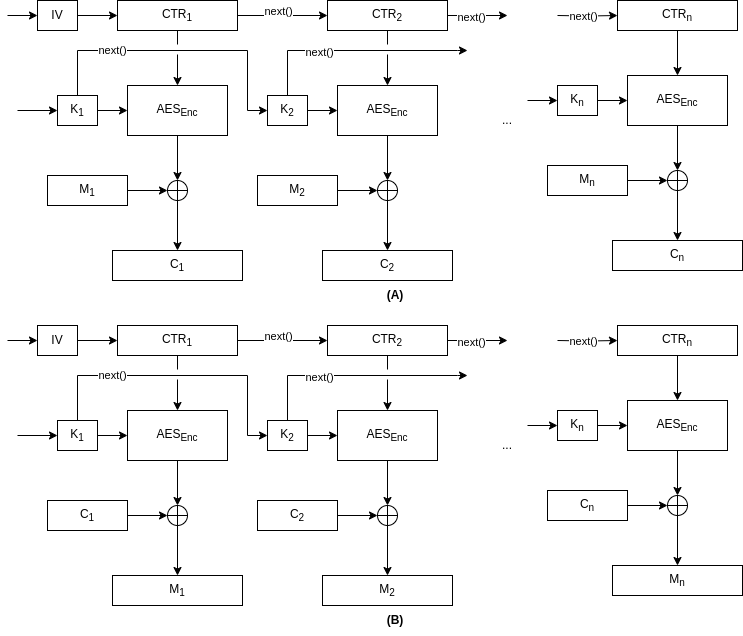
\includegraphics[width=\textwidth]{chapters/res/chapter-3/img/cipher.png}
  \caption{Ilustrasi Sistem Chaos untuk (A) Enkripsi (B) Dekripsi} \label{fig:tls.cipher}
\end{figure}

Nilai $IV$ dan $K1$ keduanya diinisialisasi berdasarkan hasil dari pertukaran kunci. Metode $\text{next}(\cdot)$ merupakan metode untuk memperbaharui sistem chaos berdasarkan persamaan \ref{eq:tls.chaos}.

Kunci MAC yang digunakan adalah kunci statis. Proses perhitungan MAC perlu melibatkan nomor frame yang digunakan sebagaimana solusi S6. Perhitungan MAC dilakukan sesuai dengan persamaan \ref{eq:tls.data.mac}.

\begin{equation}
  \label{eq:tls.data.mac}
  \begin{array}{l}
    H = \text{HMAC}(\text{key}, \text{frame\_number}\text{ }|| \\ 
      \text{   }\text{frame}.\text{type}\text{ }|| \\
      \text{   }\text{frame}.\text{version}\text{ }|| \\ 
      \text{   }\text{frame}.\text{length}\text{ }|| \\
      \text{   }\text{frame}.\text{plaintext} \\
    ) 
  \end{array}
\end{equation}

Aturan untuk pembaharuan kunci telah dijelaskan pada bagian \ref{sec:solusi.enc-dec}. Bila digambarkan melalui diagram \emph{sequence}, proses pembaharuan kunci dapat dilihat pada gambar \ref{fig:tls.cipher.update.mac.write} dan \ref{fig:tls.cipher.update.mac.read}.


\begin{figure}[!h]
  \centering
  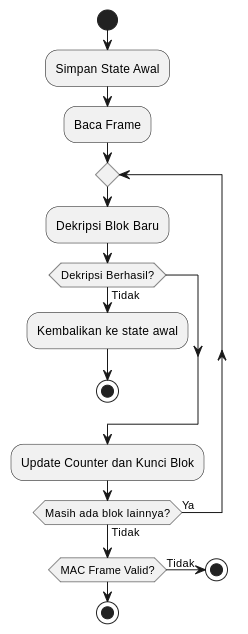
\includegraphics[width=200px]{chapters/res/chapter-3/img/update.write.png}
  \caption{Ilustrasi Proses Pembaharuan Kunci Dekripsi dan MAC pada Proses Pembacaan} \label{fig:tls.cipher.update.mac.read}
\end{figure}

\begin{figure}[!h]
  \centering
  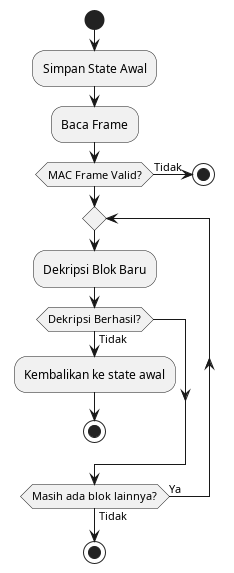
\includegraphics[width=200px]{chapters/res/chapter-3/img/update.read.png}
  \caption{Ilustrasi Proses Pembaharuan Kunci Enkripsi dan MAC pada Proses Penulisan} \label{fig:tls.cipher.update.mac.write}
\end{figure}

Pada proses enkripsi, pesan pada mulanya akan dipotong menjadi beberapa frame yang kecil. Setiap frame, akan dihitung nilai MAC dari frame tersebut lalu nilainya akan ditempelkan pada pesan. Selanjutnya, pesan akan dilakukan proses \emph{padding} dengan kelipatan 16 bytes. Hal ini agar sesuai dengan panjang blok enkripsi. Setelah pesan dilakukan \emph{padding}, tiap frame akan dilakukan operasi sebagaimana pada gambar \ref{fig:tls.cipher.update.mac.write}. Pesan yang berhasil dienkripsi akan disusun menjadi sebuah \emph{record} yang akan dikirimkan.

Pada saat menerima pesan, penerima akan melakukan proses dekripsi yang dilakukan sebagaimana pada gambar \ref{fig:tls.cipher.update.mac.read}. Setelah proses dekripsi berhasil, pesan akan dihitung MAC-nya. Bila nilai MAC valid, pesan akan digabungkan dan dilanjutkan ke \emph{layer} yang lebih tinggi. Hash yang digunakan pada MAC adalah SHA-256.

\emph{Cipher} yang dijelaskan pada bagian ini akan ditandai dengan kode \emph{cipher suite} $\text{0xff00}$ pada saat proses \emph{handshake}. Nilai awal $\text{0xff}$ berdasarkan \textcite{rfc5246} merupakan nilai yang privat sehingga dapat dijamin tidak akan bertabrakan dengan \emph{cipher suite} yang telah ada.

\subsection{Spesifikasi \emph{Handshake}}
Proses handshake dilakukan sebagaimana pada protokol TLS yang dijelaskan pada bagian \ref{sec:tls.handshake}. Proses ini dilakukan untuk membangkitkan \emph{master secret} yang digunakan. Terdapat beberapa spesifikasi khusus yang diterapkan pada protokol yang dibangun. Pertukaran kunci yang didukung hanyalah menggunakan Eliptic Curve Diffie-Hellman. Hal ini ditujukan agar keamanan dari \emph{premaster secret} dapat terjamin.

\begin{figure}[!h]
  \centering
  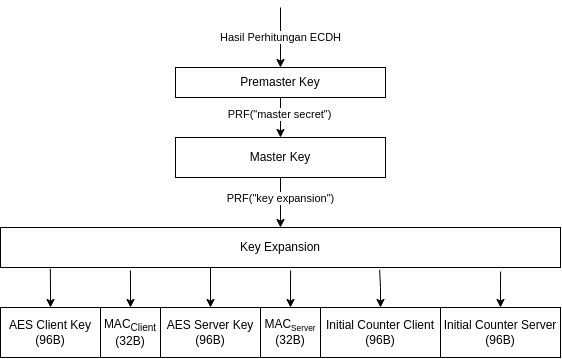
\includegraphics[width=400px]{chapters/res/chapter-3/img/keygen.png}
  \caption{Ilustrasi Pembangkitan Kunci} \label{fig:tls.keygen}
\end{figure}


Proses pembangkitan kunci diilustrasikan melalui gambar \ref{fig:tls.keygen}. Hasil dari proses Eliptic curve Diffie-Hellman akan menghasilkan \emph{premaster secret}. Saat \emph{premaster secret}, kunci \emph{master secret} akan dihasilkan melalui fungsi PRF. Saat \emph{master secret} berhasil dibangkitkan, perlu dilakukan proses \emph{key expansion}. Panjang kunci yang harus diekspansi adalah 448 bytes. Hal ini dikarenakan diperlukannya empat pasang sistem \emph{chaos} yang digunakan untuk pembangkitan sistem chaos dan dua buah kunci MAC. Tiap sistem \emph{chaos} memerlukan tiga buah parameter sehingga dibutuhkan 96 bytes per sistem \emph{chaos}. Ilustrasi dari ekspansi kunci dapat dilihat pada gambar \ref{fig:tls.keyexpansion}.

\begin{figure}[!h]
  \centering
  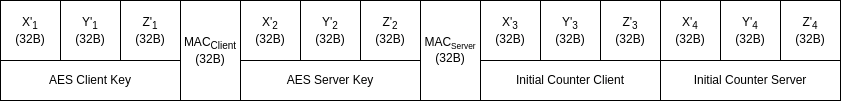
\includegraphics[width=400px]{chapters/res/chapter-3/img/keyexpansion.png}
  \caption{Ilustrasi Ekspansi Kunci} \label{fig:tls.keyexpansion}
\end{figure}

Persamaan \ref{eq:tls.key.convert} menunjukkan proses pengubahan kunci yang dilakukan menjadi parameter chaos. $K$ adalah potongan kunci dari hasil ekspansi.

\begin{equation}
  \begin{aligned}
    X_i = f(X'_i) \\
    Y_i = f(Y'_i) \\
    Z_i = f(Z'_i) \\
    E_i = (X_i, Y_i, Z_i)
  \end{aligned}
  \label{eq:tls.key.convert}
\end{equation}

Tabel \ref{tab:tls.keyexpansion} menunjukan kegunaan dari setiap hasil ekspansi kunci yang dilakukan. Tabel tersebut menjelaskan nilai awal dari sistem \emph{chaos} yang digunakan untuk pembangkitan kunci blok, kunci MAC, dan nilai IV.

\begin{table}[!h]
  \centering
  \caption{Parameter Hasil Ekspansi Kunci} \label{tab:tls.keyexpansion}
  \begin{tabular}{|p{3cm}|p{3cm}|p{6cm}|}
    \hline
    \textbf{Nama Parameter} & \textbf{Variabel} & \textbf{Deskripsi} \\
    \hline
    \emph{MAC Client Key} & $\text{MAC}_1$ & Nilai Kunci MAC yang digunakan oleh client \\ \hline
    \emph{MAC Server Key} & $\text{MAC}_2$ & Nilai Kunci MAC yang digunakan oleh server \\ \hline
    \emph{AES Client Key}  & $E_1$ & Nilai awal  parameter \emph{chaos} yang digunakan client untuk melakukan enkripsi ($K_1$) \\ \hline
    \emph{AES Server Key}  & $E_2$ & Nilai awal parameter \emph{chaos} yang digunakan server untuk melakukan enkripsi ($K_1$) \\ \hline
    \emph{Initial Counter Client}  & $E_3$ & Nilai \emph{counter} awal yang digunakan client untuk enkripsi \\ \hline
    \emph{Initial Counter Server}  & $E_4$ & Nilai \emph{counter} awal yang digunakan server untuk enkripsi \\
    \hline
  \end{tabular}
\end{table}

\subsection{Spesifikasi Pengiriman Pesan}

Pada proses pengiriman pesan, pesan terlebih dahulu dilakukan operasi kriptografi sebagaimana penjelasan pada bagian \ref{sec:solusi.enc-dec}. Setelah itu, pesan akan disusun menjadi sebuah \emph{record} yang akan dikirimkan. Gambar \ref{fig:tls.application.rec} menunjukkan protokol record yang digunakan untuk mengirimkan pesan.

\begin{figure}[!h]
  \centering
  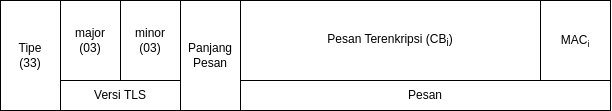
\includegraphics[width=\textwidth]{chapters/res/chapter-3/img/tls.application.record.png}
  \caption{Ilustrasi \emph{Application Record} yang digunakan} \label{fig:tls.application.rec}
\end{figure}

Berdasarkan \textcite{rfc5246}, Nilai tipe haruslah 33. Hal ini menyatakan bahwa pesan yang dikirimkan merupakan \emph{Application Data}. Nilai \emph{version} yang digunakan adalah $\text{0x0303}$. Hal ini menyatakan protokol yang digunakan adalah TLSv1.2. Panjang pesan ($L$) merupakan panjang dari pesan dan MAC dalam keadaan terenkripsi. Secara matematis dihitung berdasarkan persamaan \ref{eq:tls.record.length}.

\begin{equation}
  \begin{aligned}
    L = \text{len}(CB_{i})
  \end{aligned}
  \label{eq:tls.record.length}
\end{equation}

Blok pesan terenkripsi merupakan hasil dari proses enkripsi yang dilakukan pada bagian \ref{sec:solusi.enc-dec}. Blok tersebut berisi informasi terkait dengan \emph{plaintext} dan MAC dalam keadaan terenkripsi. Hal ini dilakukan untuk mencegah adanya serangan \emph{side-channel} dengan mengamati waktu dekripsi pesan.
